
\chapter{Оптимизация конструкции робота}\label{ch:ch2}

Вторая глава покрывает разработку объекта исследования, а именно решение задачи структурного синтеза и инженерную разработку прототипа.

\section{Решение задачи структурного синтеза}

Для эффективного исследования пещер необходимо выставить требования к разрабатываемому роботу. На основании литературного обзора было решено, что робот должен:
\begin{enumerate}
    \item иметь малые габариты, чтобы иметь возможность пролезать через щели в скальной породе и не застревать среди камней;
    \item обладать достаточной проходимостью по сыпучим грунтам;
    \item иметь возможность преодолевать малые водные преграды;
    \item мог взбираться на большие каменные уступы.
\end{enumerate}

Было решено, что цикловой движитель с одной степенью свободы в ноге лучше всего подходит для решения подобных задач.

Для цикловых движителей с одной степенью свободы в ноге вопрос о количестве ног не имеет однозначного решения. Поэтому необходимо провести структурный синтез, чтобы определить их количество. Данная задача решалась с помощью генетического алгоритма.

Генетический алгоритм это эвристический алгоритм поиска, используемый для решения задач оптимизации и моделирования путём случайного подбора, комбинирования и вариации искомых параметров с использованием механизмов, аналогичных естественному отбору в природе. Для решения задачи использовалась библиотека Deap.

Для создания подходящего робота, который может эффективно решать конкретные задачи, необходимо провести структурный синтез. Это означает, что мы оптимизируем такие характеристики робота, как количество ног, угол между ногами и т.д., используя алгоритмы оптимизации. Обычно в алгоритмах оптимизации оптимизируется фитнес или объективная функция. 

При оптимизации очень важно выбрать подходящую функцию пригодности. Иногда эта функция может быть явно выражена через аналитическую формулу: например, выражение общего материального объема робота как функции его геометрических параметров. Однако в других случаях желаемая мера эффективности не может быть вычислена в явном виде и может быть получена только с помощью физического эксперимента или соответствующего моделирования. В нашем случае мы стремимся максимизировать ходовые качества робота на различных сложных участках, и основным используемым показателем будет проходимость местности. Таким образом, мы автоматически создадим симулированные версии нашего робота, используя различные варианты параметров проектирования, а также симулированные версии различных типов местности: а затем мы оценим пригодность робота для ходьбы с помощью физической симуляции, во время которой робот будет проходить по местности. Также были получены параметризации различных генеративных моделей местности, чтобы мы могли на более позднем этапе исследовать влияние не только типа местности, но и параметров местности на возможность появления многоножек, и, следовательно, на лучшие конструкции в зависимости от конкретной местности.

Для того чтобы направлять процесс поиска в пространстве возможных значений параметров, мы решили использовать модифицированный эволюционный алгоритм, который создает последовательные поколения конструкций с помощью соответствующих генетических операторов, играющих роль мутаций и скрещивания. После нескольких инициализаций и поколений были получены многообещающие результаты и полезные идеи, которые позволили нам создать конструкции, значительно улучшающие производительность, для достижения нашей конечной цели - многоножек, способных преодолевать сложные участки местности. Такие роботы необходимы во многих областях применения, включая поиск и спасение (хождение по обломкам разрушенных зданий), преодоление неровных скалистых и горных местностей для мониторинга окружающей среды и логистики, и многое другое. 

Полный текст статьи можно прочитать \cite{bulichevOptimizationCentipedeRobot2017}.

Геометрическая модель робота представлена в виде трехмерного параллелепипеда. Количество движителей по каждому из бортов обозначается через $\gamma$. Разность фаз между соседними движителями обозначается через  $\alpha$ \pic{fig:best_gen_robot.jpg}.

\begin{figure}[H]
    \centering
    \begin{tikzpicture}
        % Include the image in a node
        \node [above right, inner sep=0] (image) at (0,0)
        {\centering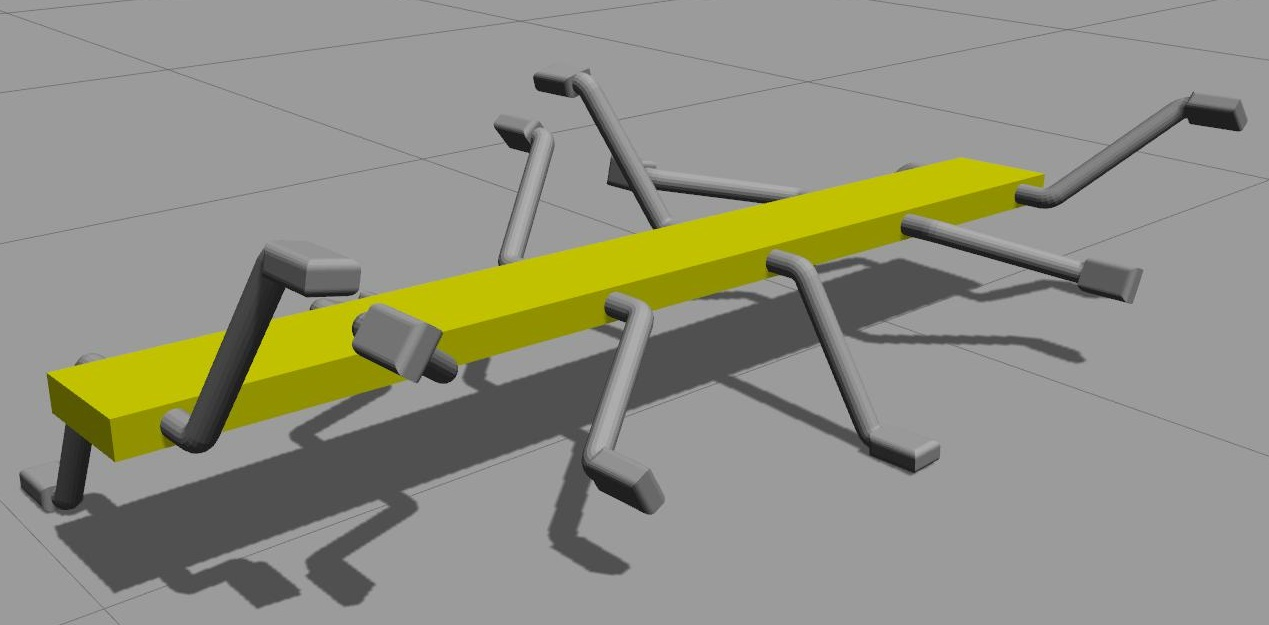
\includegraphics[height=10cm,width=1\textwidth,keepaspectratio]{best_gen_robot.jpg}};
        % Create scope with normalized axes
        \begin{scope}[
                x={($ 0.1*(image.south east)$)},
                y={($ 0.1*(image.north west)$)}]
            % Labels
            \draw [green, very thick,
                decorate,
                decoration = {brace,
                        raise=5pt,
                        amplitude=5pt,
                        aspect=0.5}] (1.4,3.6) --  (8.1,6.8)
            node[rounded corners=3pt, pos=0.5,above left =14pt,black,fill=white]{\tiny $(\gamma - 1) h_{\text{leg}}sin(\alpha)$};

            \draw[stealth-, very thick,green] (9.5,7.8) -- (7.8,1.94);
            \draw[stealth-, very thick,green] (1.5,2.8) -- (7,1)
            node[rounded corners=3pt,right,black,fill=white]{\tiny $\gamma = 6$};

            \draw[thin,green] (6.7,4) -- (5.75,9);
            \draw[thin,green] (4.85,3.5) -- (5.75,9);
            \draw[thin,green,stealth-stealth] (6.32,6) arc (-79.2:-99.2:3) node [rounded corners=3pt,below = 2pt,black,fill=white, midway] {\tiny $\alpha$};
        \end{scope}
    \end{tikzpicture}
    \caption{Схема модели робота для генетического алгоритма}
    \label{fig:best_gen_robot.jpg}
\end{figure}

Эту задачу можно сформулировать как мультикритериальную задачу оптимизации, где необходимо максимизировать дистанцию, пройденную за фиксированное время, и минимизировать длину робота \eqref{eq:second}. Параметрами индивида являлись $\gamma$ и $\alpha$.

\begin{eqnarray}
    \label{eq:second}
    F \rightarrow max = \beta \left( {\omega}_{1} \cdot \overbrace{\delta}^{\text{Distance}} + {\omega}_{2} \cdot \overbrace{\frac{1}{(\gamma - 1) h_{\text{leg}}sin(\alpha)}}^{\text{Simplified body length}}\right) + \\ \nonumber + (1 - \beta) {\delta}^{{\omega}_{1}} {\left( \frac{1}{(\gamma - 1)h_{\text{leg}}sin(\alpha)}\right)}^{{\omega}_{2}}
\end{eqnarray}
где \nom{$\delta$}{пройденная дистанция}, \nom{$\beta$}{адаптивный параметр}, \nom{${\omega}_{1,2} \in  [ 0..1 ] $}{весовые коэффициенты}.


Модель робота должна быть реализована в формате URDF. Это язык разметки формата XML для представления модели робота. Но это старый формат, и когда модель импортируется в Gazebo, URDF преобразуется в формат SDF. Это важно, потому что некоторые функции не реализованы в чистом URDF. В нашем случае это шарнир коробки передач. Но можно вставить код в формат SDF, и он будет работать правильно.

\subsection{Генерирование местности, над которой будет проходить робот}
В основе нашего решения лежит пятый подход (представленный в справочном разделе данной работы).
Параметры местности, которые могут быть изменены, следующие:
\begin{itemize}
\item номер ширины и длины клетки;
\item диапазон высоты клетки начало и конец;
\item ширина и длина клетки;
\item 2(3) измерения местности (рис.~\ref{fig:terrain_1});
\item параметр распределения (рис.~\ref{fig:terrain_2}).
\end{itemize}

Для выбора высоты клеток были проведены эксперименты.
Существует 3 диапазона, определяющих свойства местности, которые изображены ниже (рис.~\ref{fig:range}).

\begin{figure}[H]
\centering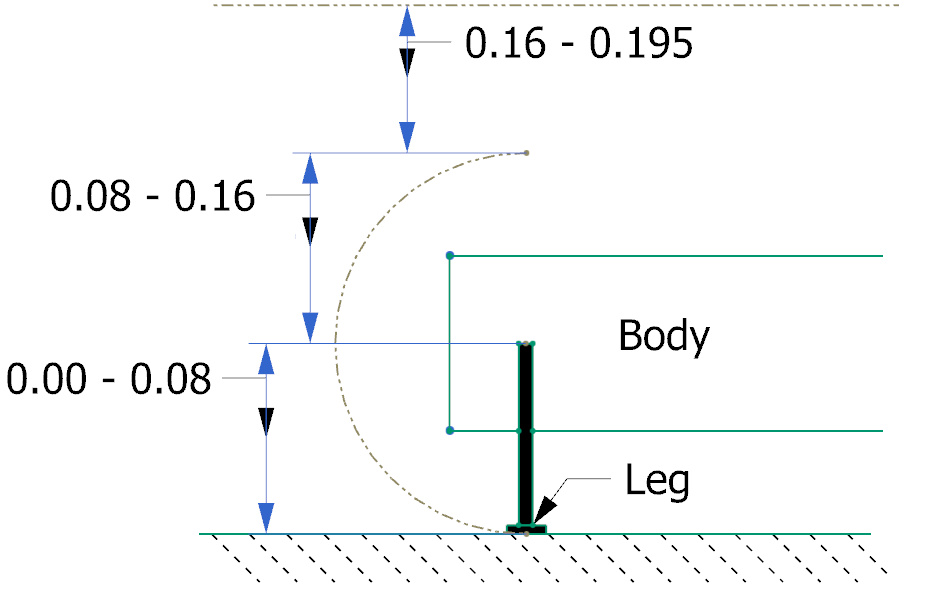
\includegraphics[width=0.5\textwidth]{from_master/ranges}\\
\caption{Три диапазона для оценки рельефа местности}
\label{fig:range}
\end{figure}

Для каждого полигона было сгенерировано 20 местностей и 50 роботов. Каждый робот пытается пройти все местности. У робота есть 4 секунды моделирования и он пытается пройти первое препятствие. Успешные попытки засчитывались. Результаты можно увидеть в таблице \ref{tabular:ranges}.

\begin{table}[H]
\caption{Процентное соотношение между диапазонами и успешными попытками}
\label{tabular:ranges}
\begin{center}
\begin{tabular}{c|c}
 \textbf{Range} & \textbf{Percentage}\\
 \hline
0.00 -- 0.08 & 99.7 \\ 
0.08 -- 0.16 & 79.7 \\
0.16 -- 0.195 & 47.3 \\
\end{tabular}
\end{center}
\end{table}


Таким образом, было решено, что второй \& первый диапазоны (0.00 - 0.16) будут использоваться в алгоритме оптимизации, чтобы иметь дело со средне-жесткими грунтами.

В информатике генетические алгоритмы - это адаптивные эвристические алгоритмы поиска, основанные на эволюционных концепциях. Они представляют собой интеллектуальную параллельную эксплуатацию пространства проектирования и могут быть использованы для решения проблем оптимизации, не обязательно оптимизируя, но часто получая близкие к оптимальным решения. 

Была выбрана библиотека Deap \cite{fortin2012deap}, поскольку в ней есть все необходимые инструменты для реализации поставленной задачи.

После случайной генерации начальной популяции, алгоритм эволюционирует с помощью трех операторов:
\begin{enumerate}
\item Selection (основанный на повышенной вероятности выживания сильнейшего);
\item Кроссинговер (который представляет собой спаривание между особями);
\item Мутация (которая вносит случайные изменения).
\end{enumerate}

Оператор Selection был взят из библиотеки Deap. Он использует турнирный подход.
Однако в библиотеке Deap мы написали собственные реализации кроссовера и мутации:
\begin{enumerate}
\item Crossover: мы используем общую функцию с некоторыми дополнениями. Каждая особь имеет 4 поля, но четвертое поле (расстояние) зависит от других полей. Поэтому наша функция кроссинговера должна работать только с первыми тремя характеристиками.

\item Mutation: Аналогично Crossover, здесь мы работаем только с тремя полями: количество ног, угол между двумя соседними ногами и волновое смещение между сторонами. Наша модель имеет ограничения по максимальной длине и т.д., поэтому с некоторой заданной вероятностью каждая из характеристик может быть изменена в определенном интервале. Мутация может произойти один или два раза, но вероятность уменьшается. Это означает, что если произошла первая мутация, то вероятность для этой особи становится ниже. 
\end{enumerate}

Этот псевдокод дает высокоуровневое описание всего алгоритма.

\begin{algorithm}[h]
\caption{Верхеуровневый генетический алгоритм\label{high_level}}
% \begin{small}
\KwIn{$\alpha$ -- number of generations, $\beta$ -- number of individuals, $\gamma$ -- number of terrains}
\KwOut{Good enough parameters for robot}
\Begin{
generate set of terrains\;
randomly initialize a first population of robots\;
\For{$i = 0$ \KwTo $\alpha$}{
\For{$j = 0$ \KwTo $\beta$}{
$distance = 0$\;
\For{$k = 0$ \KwTo $\gamma$}{
start simulation\;
$distance += cur\_distance$\;
}
$avg\_distance = distance / \gamma$\;
evaluate fitness function\;
}
select the best parents\;
perform crossover on chosen parents\;
perform mutation\;
}
}
% \end{small}
\end{algorithm}

Результаты были получены на двух этапах. На первом этапе мы стремились найти только одного лучшего робота, только для местности T1. На втором этапе мы хотели увидеть зависимость производительности от повторной инициализации эксперта, и, что самое важное, от различных типов местности. 

Первая фаза: Каждый робот прошел 10 различных рельефов и потратил на каждый по 9 секунд.
В результате нашей работы мы получили следующие результаты: после 11 поколений и 200 особей в начальной популяции лучший робот имеет по 6 ног с каждой стороны (всего 12 ног), угол между ногами 73 градуса и волновое смещение между сторонами 163 градуса. С такими характеристиками робот смог пройти 5,21 метра, в то время как начальная популяция могла пройти менее 2. На рисунке ниже \pic{fig:best_robot} показан лучший робот, найденный на первом этапе. На следующем рисунке \pic{fig:plot4} показаны траектории улучшения приспособленности для первой фазы экспериментов, показывающие приспособленность max, min, avg + std, avg - std, в разных поколениях. 


\begin{figure}[H]
\centering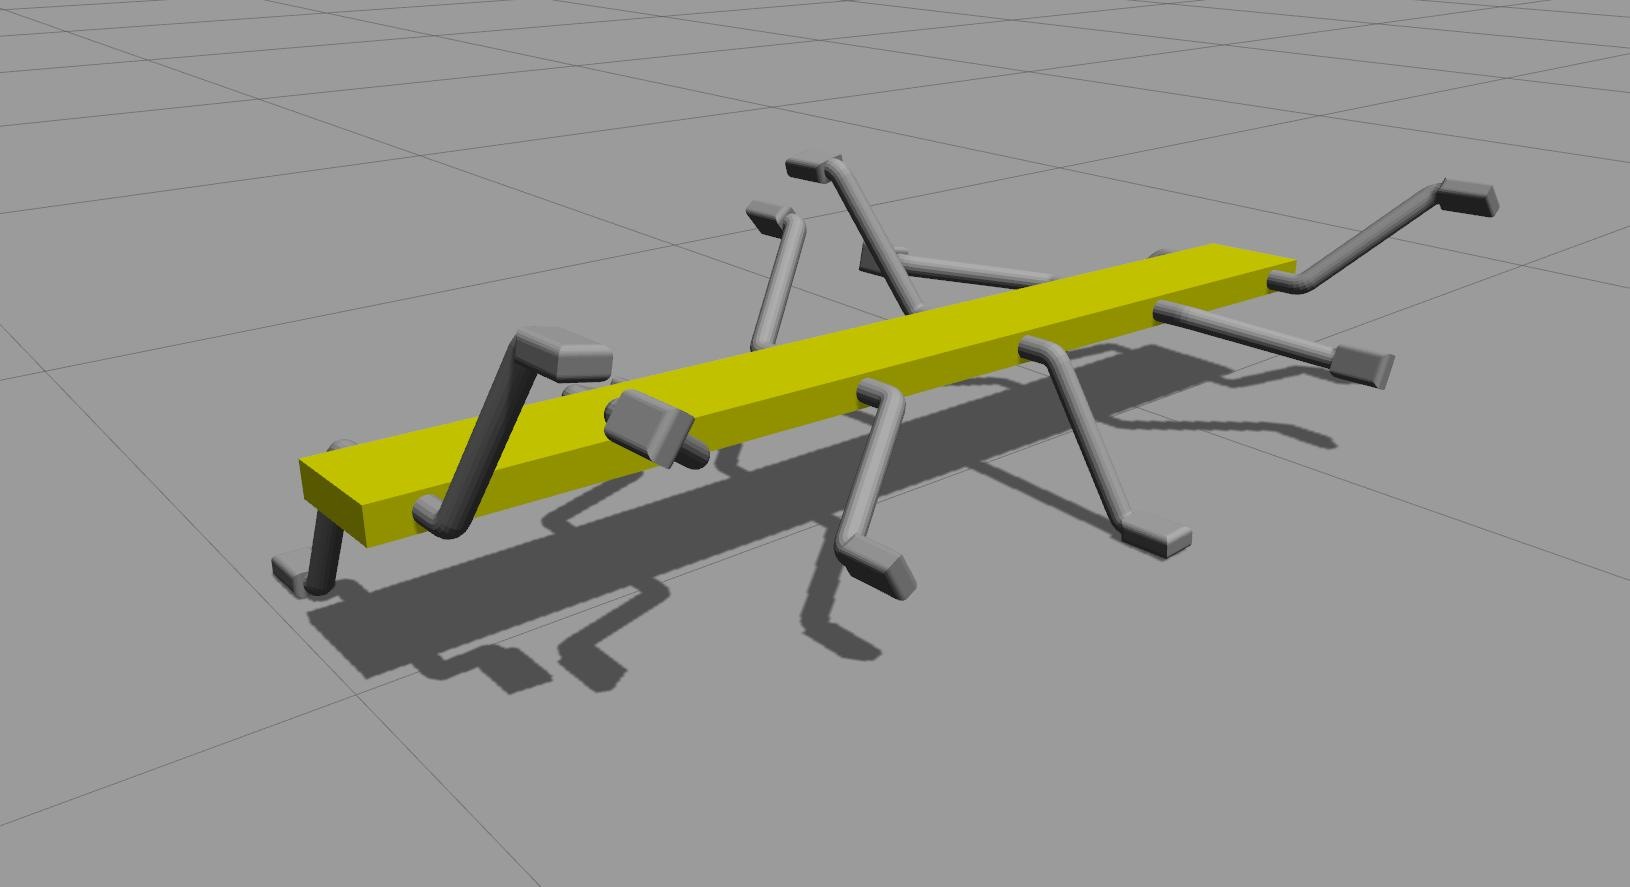
\includegraphics[width=0.4\textwidth]{from_master/best_robot}\\
\caption{Робот с результирующими результатами}
\label{fig:best_robot}
\end{figure}
\begin{figure}[H]
\centering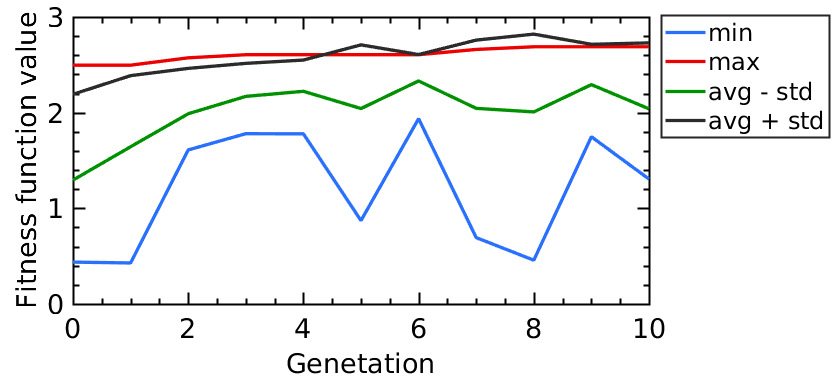
\includegraphics[width=0.6\textwidth]{from_master/best_robot_200_plot}\\
\caption{Среднее значение фитнес-функции $\pm$ std на поколение
Минимальное и максимальное значения фитнес-функции на поколение}
\label{fig:plot4}
\end{figure}

Вторая фаза: Для каждого из трех типов местности используются следующие параметры:
\begin{itemize}
\item 11 поколений;
\item 55 особей;
\item 10 различных местностей и 9 секунд;
\item 9 секунд на каждой местности.
\end{itemize}

Весовые коэффициенты настраивались в зависимости от выбора приоритета. Невзирая на выбранные коэффициенты, оптимальным набор ног начинался с 8 и заканчивался 14. Это объясняется критерием статического равновесия, который, как оказалось, увеличивает проходимость механизма. В данном случае 4 ноги всегда будут касаться пола. 

Было проведено два испытания. На первом испытании мы стремились найти только одного лучшего робота, только для местности T1 \pic{fig:terrain_1}. На втором этапе мы хотели видеть зависимость от разных типов ландшафтов при меньшем количестве индивидуальностей.

Первый этап: каждый робот проходил 10 разных ландшафтов по 9 секунд каждую. Вторая фаза: она имеет те же параметры, что и первая фаза, но с измененным размером популяции. 

В соответствии с таблицей \ref{tabular:Table2} (весовые коэффициенты равны 0.6 и 0.4 соответственно) видно, что мы имеем сходимость в параметрах. Видео прохождения препятствия лучшим индивидом \quad
\qrcode[height=1.5cm]{https://youtu.be/DcovvkTZgsg}

\begin{figure}[h]
    \begin{subfigure}{0.33\textwidth}
    \centering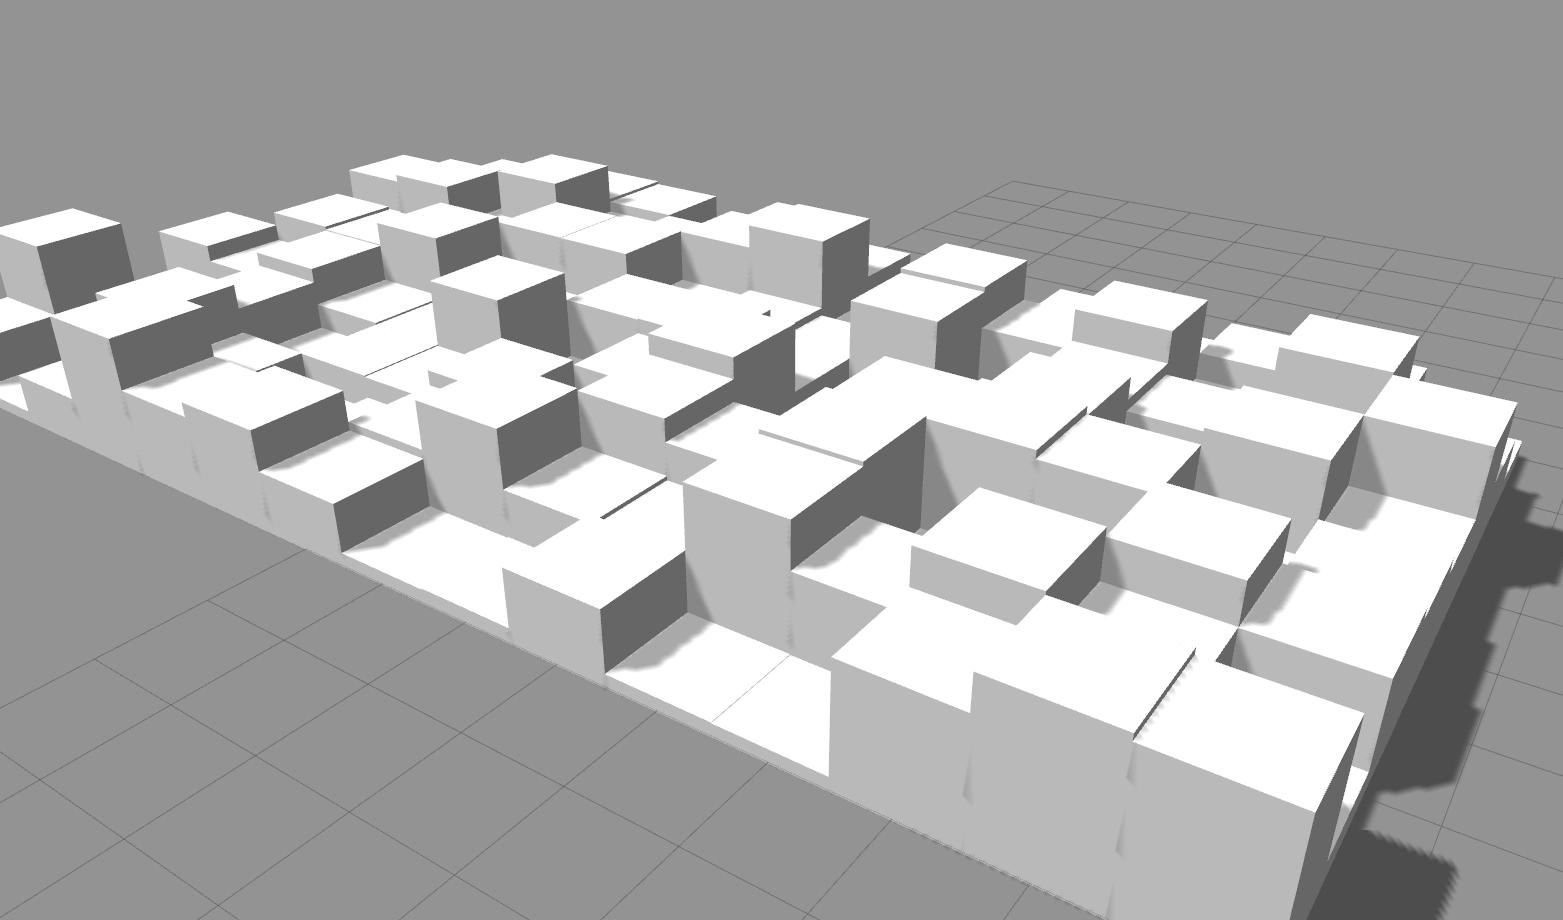
\includegraphics[width=0.8\textwidth]{terrain_1} 
    \caption{T1: 3D-боксы с равномерным распределением высоты}
    \label{fig:terrain_1}
    \end{subfigure}
    \begin{subfigure}{0.33\textwidth}
    \centering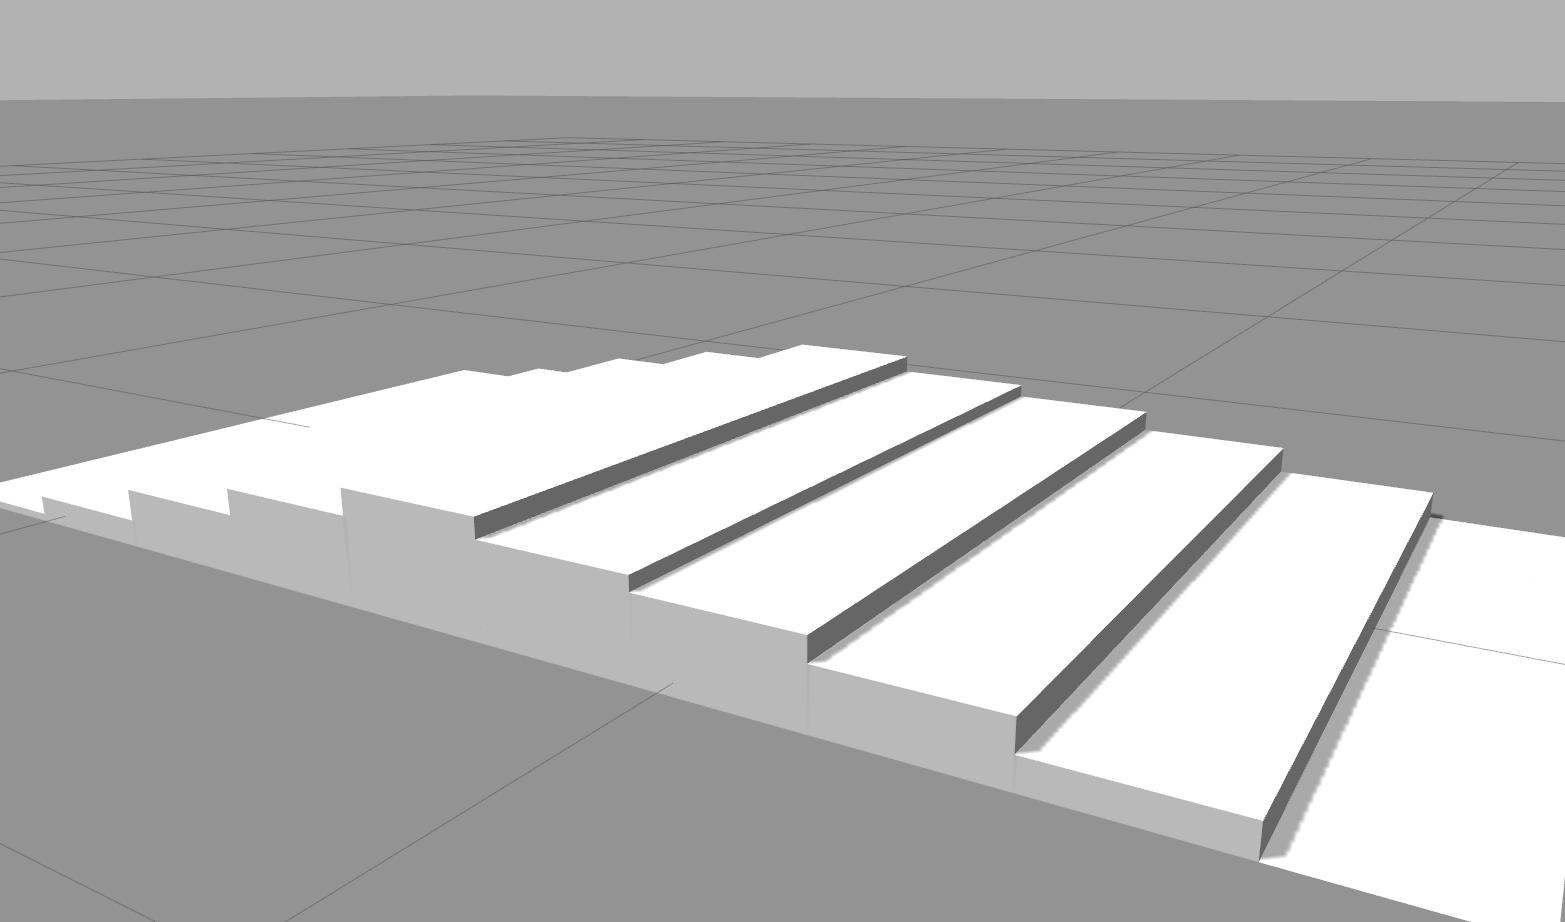
\includegraphics[width=0.8\textwidth]{terrain_2} 
    \caption{T2: 2D-полосы с гауссовой функциональной высотой}
    \label{fig:terrain_2}
    \end{subfigure}
    \begin{subfigure}{0.33\textwidth}
    \centering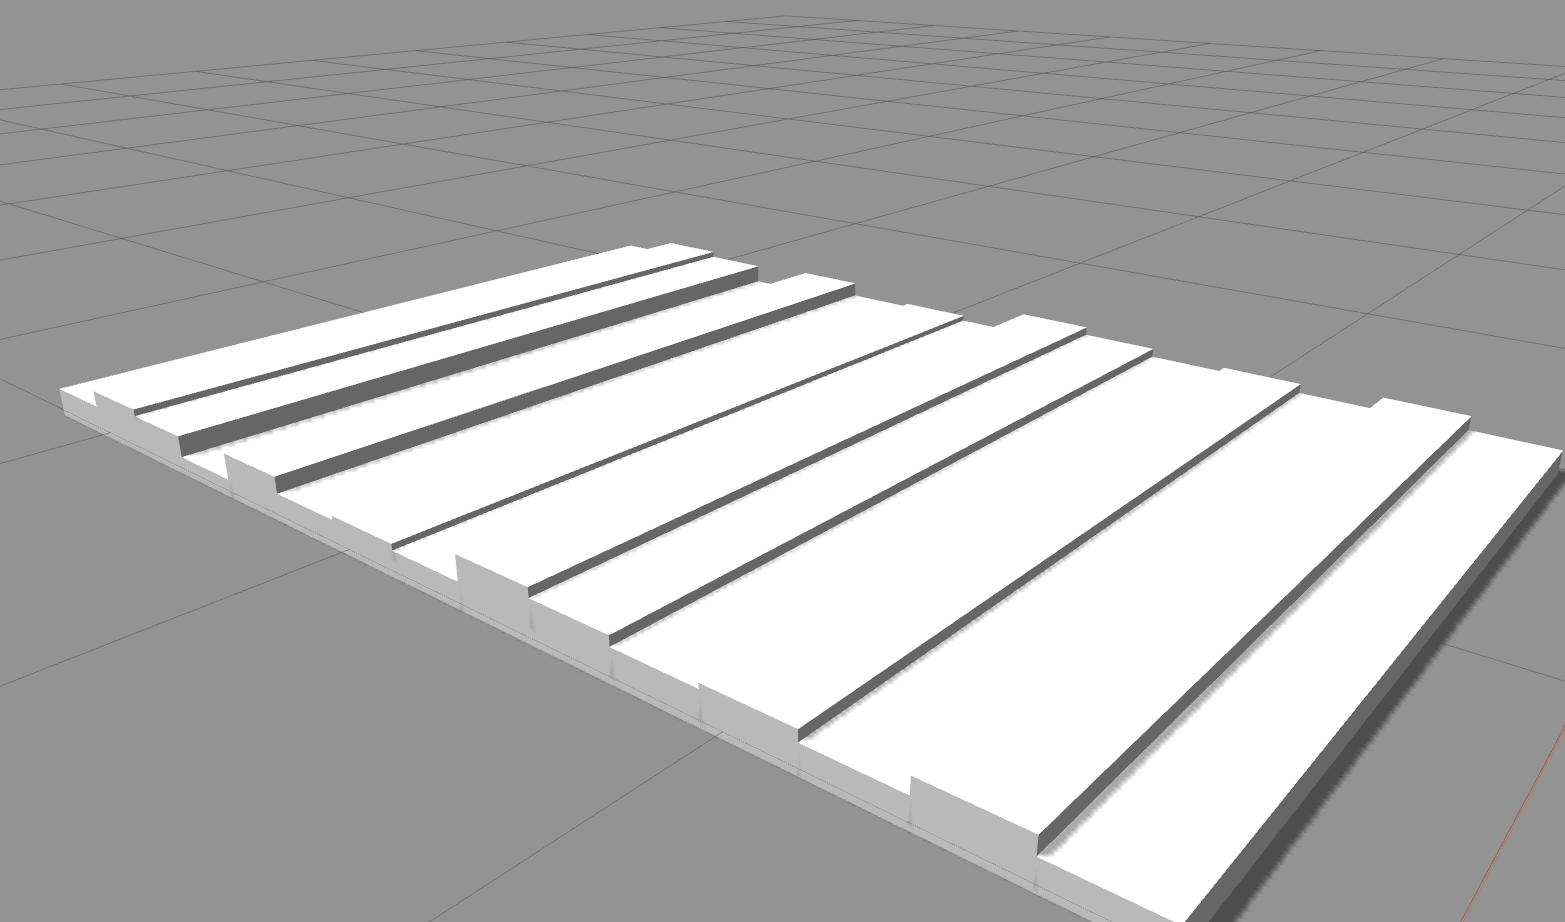
\includegraphics[width=0.8\textwidth]{terrain_3}
    \caption{T3: 2D-полосы с распределением высоты по гауссовской функции)}
    \label{fig:terrain_3}
    \end{subfigure}
     
    \caption{Примеры сгенерированных территорий}
    \label{fig:terrains}
\end{figure}
\vspace{-0.5cm}

\begin{table}[H]
\caption{Зависимость между статистикой значения пригодности и типами ландшафта}
\label{tabular:Table2}
\begin{center}
\begin{tabular}{c|c|c|c}

\textbf{\makecell{Территория, популяция}} & \textbf{\makecell{Параметры}} & \textbf{\makecell{Среднее \\значение }} & \textbf{\makecell{Std \\целевая функция}}\\
\hline
\textbf{\makecell{T1 \pic{fig:terrain_1}, 110}} & \makecell{(6, 72)} & \makecell{2.38} & \makecell{0.34}
\\
\textbf{\makecell{T2 \pic{fig:terrain_2}, 55}}& \makecell{(5, 68)} & \makecell{1.95} & \makecell{0.35} 
\\
\textbf{\makecell{T3 \pic{fig:terrain_3}, 55}} & \makecell{(6, 77)} &  \makecell{2.08} & \makecell{0.33} \\
\hline
\end{tabular}
\end{center}
\end{table}

\section{Решение задачи на основе кинематики}
Этот тип робота имеет некоторые проблемы, одна из которых - колебания. В результате управление становится сложным и неточным.
Поэтому, чтобы преодолеть эту проблему, мы можем частично решить ее путем изменения угла между соседними ногами.

Далее следует наша целевая функция. Мы должны максимизировать положение Z и минимизировать STD. Одновременно мы должны минимизировать RMS и std углы в обоих направлениях (крен и тангаж). Важным моментом является и направление движения.

Объективная функция имеет следующий вид:
\begin{eqnarray}
    \label{eq:objective}
    F = \sum\limits_{i=1}^4 \omega_{i} \cdot (\frac{1}{\omega_{z1}Z_{rms}^i - \omega_{z2}Z_{std}^i}  + ( \omega_{p1}\alpha_{rms}^i + \omega_{p2}\alpha_{std}^i) + \nonumber \\\ + (\omega_{r1}\beta_{rms}^i + \omega_{r2}\beta_{std}^i)) \rightarrow min
\end{eqnarray}
где надпись \nom{$i =\{1,2,3,4\}$}{среднее значение a, которое принимается из 1 - движение вперед, 2 - движение влево, 3 - движение вправо, 4 - вращение}; \nom{$Z$}{положение по оси Z}; \nom{$\alpha, \beta$}{значения ориентации по крену и шагу}; \nom{$\omega_{i}$}{весовой коэффициент для каждого направления}, \nom{${\omega}_{z,roll,pitch}$}{весовые коэффициенты}.

В нашем случае мы можем просто найти все возможные решения за неподходящее время, потому что нам нужно только проверить 36 углов ~$\cdot$ 4 направления ~$\cdot$ 100 экспериментов для каждого направления ~$\cdot$ 144 шага в каждом.


Есть пример, который описывает два возможных движения: вперед и скольжение. Результаты о положении почти одинаковы для обоих типов, и я сделал рисунок только для движения вперед.

\begin{figure}[H]
\begin{subfigure}{1\textwidth}
\centering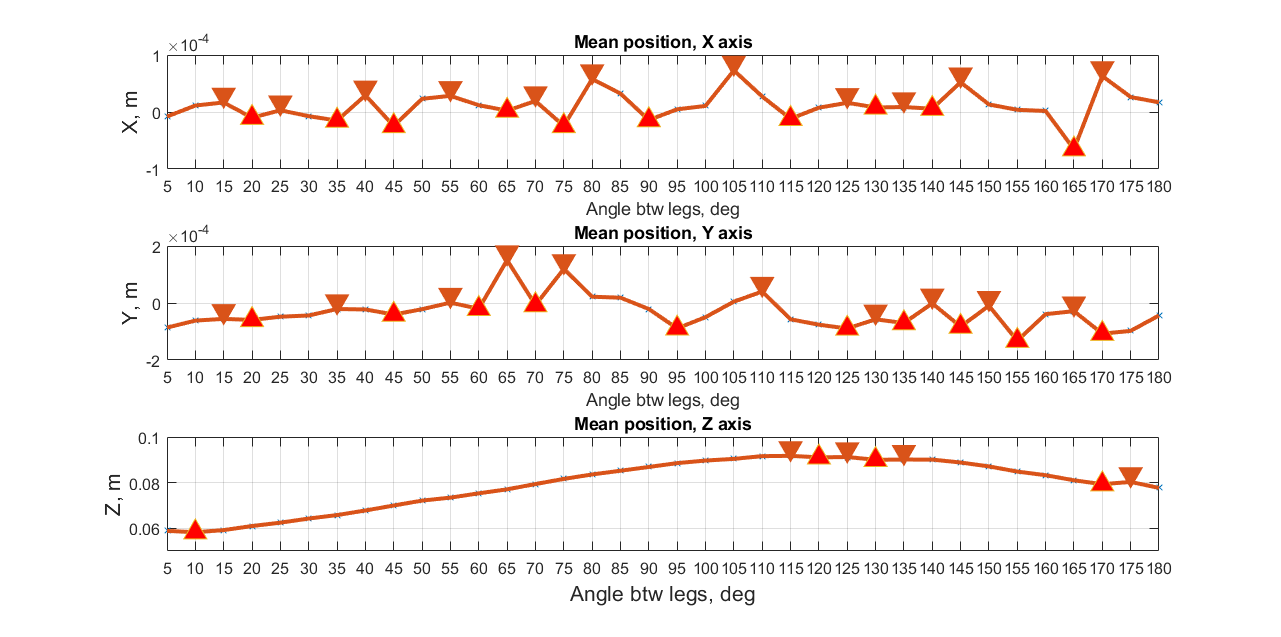
\includegraphics[width=0.8\textwidth]{from_master/forwardBestMean} 
\caption{Среднее значение из данных о положении для обоих типов движения}
\label{fig:forwardBestMean}
\end{subfigure}

\begin{subfigure}{1\textwidth}
\centering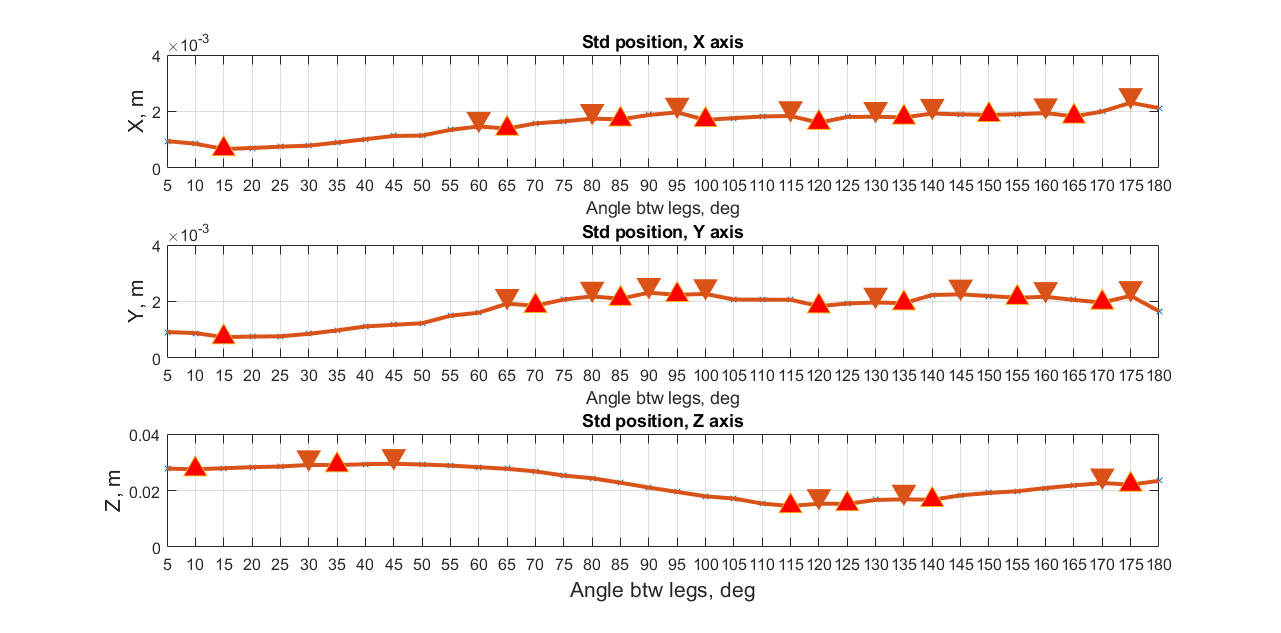
\includegraphics[width=0.8\textwidth]{from_master/forwardBestSTD} 
\caption{STD из данных о положении для обоих типов движения}
\label{fig:forwardBestSTD}
\end{subfigure}
 
\caption{Данные о положении для обоих типов движения}
\label{fig:forwardPosion}
\end{figure}

\begin{figure}[H]
\centering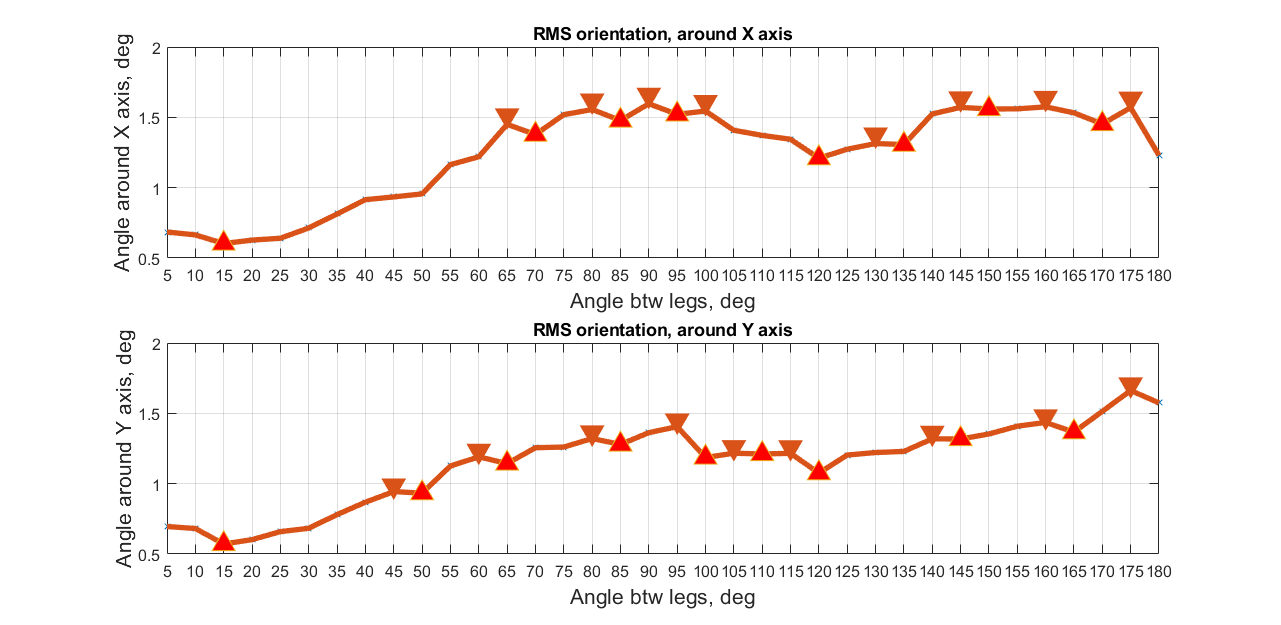
\includegraphics[width=0.8\textwidth]{from_master/forwardBestRMSrot} 
\caption{RMS из данных об ориентации для типа движения вперед}
\label{fig:forwardBestRMSrot}
\end{figure}

\begin{figure}[H]
\centering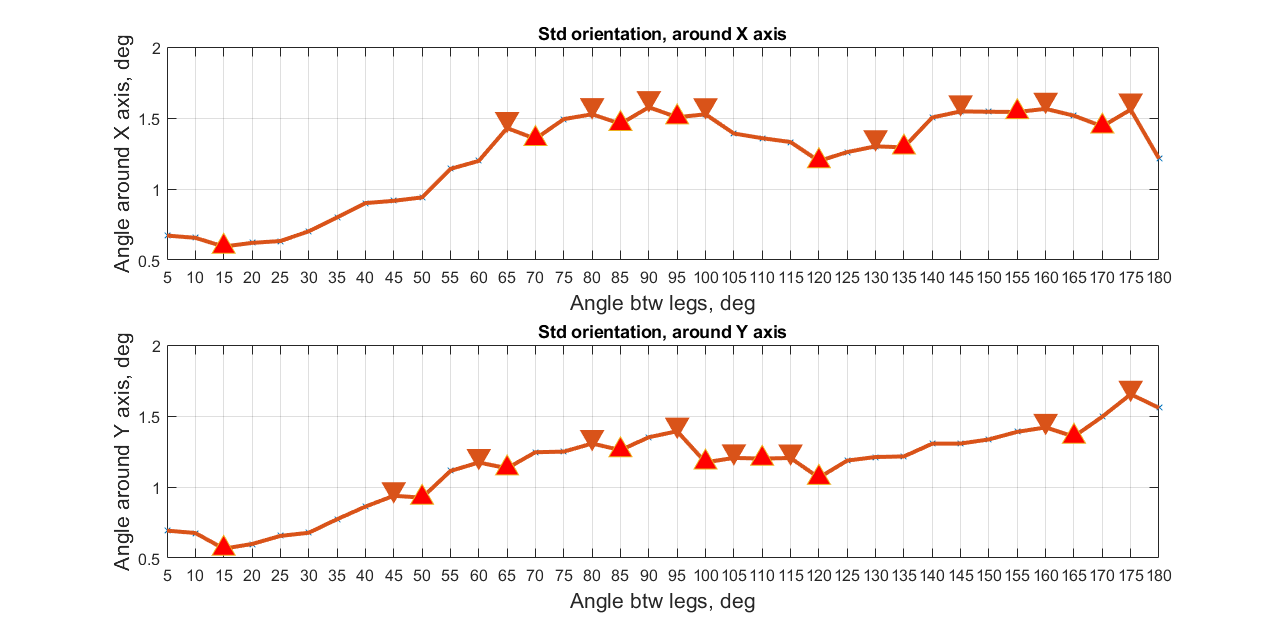
\includegraphics[width=0.85\textwidth]{from_master/forwardBestSTDRot} 
\caption{STD из данных об ориентации для типа движения вперед}
\label{fig:forwardBestSTDRot}
\end{figure}

\begin{figure}[H]
\begin{subfigure}{1\textwidth}
\centering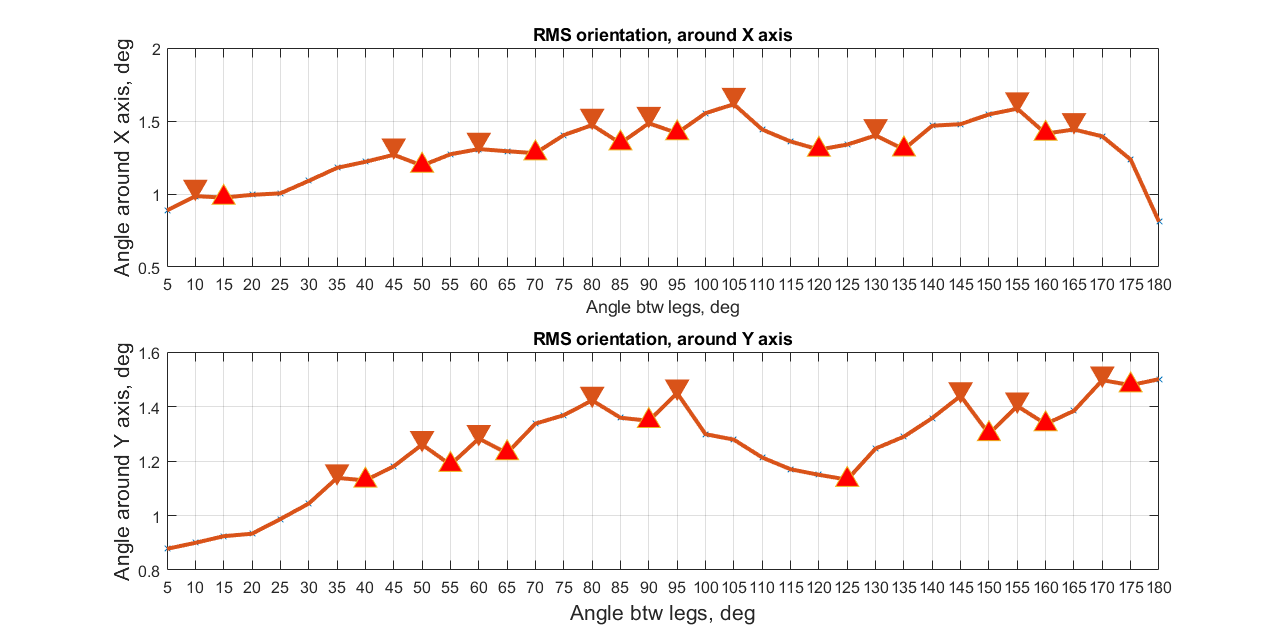
\includegraphics[width=0.8\textwidth]{from_master/slideBestRMSrot} 
\caption{RMS из данных об ориентации для типа движения вбок}
\label{fig:slideBestRMSrot}
\end{subfigure}

\begin{subfigure}{1\textwidth}
\centering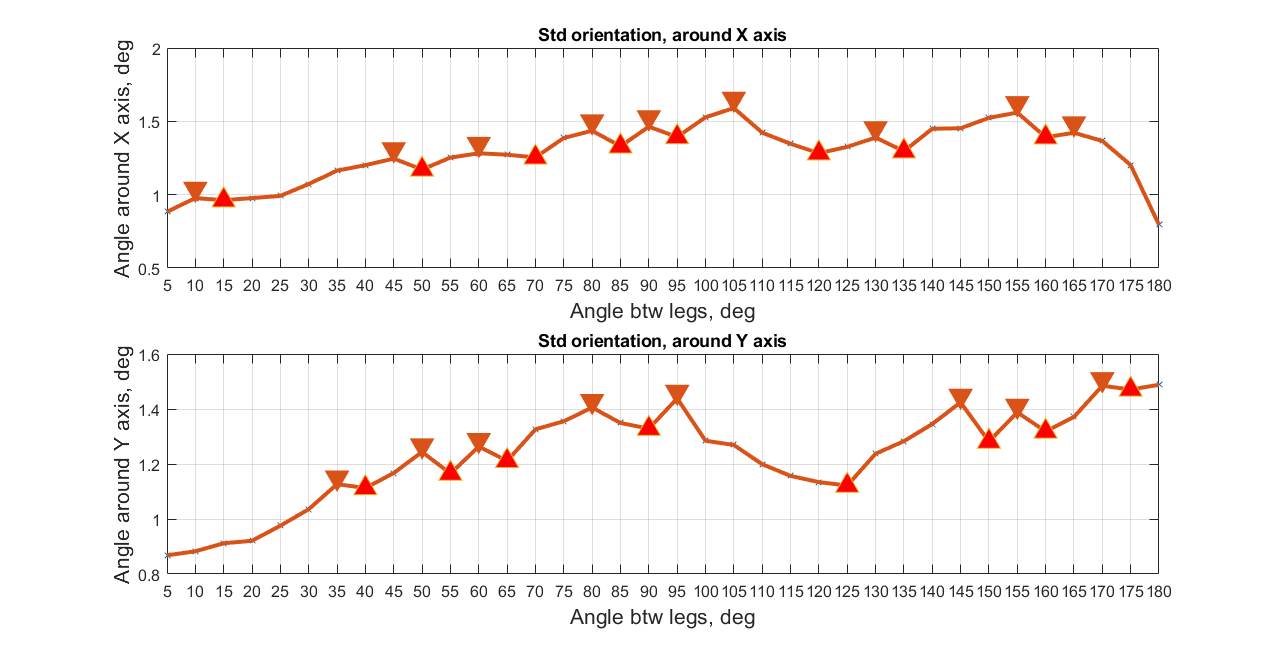
\includegraphics[width=0.8\textwidth]{from_master/slideBestSTDRot} 
\caption{STD из данных об ориентации для типа движения вбок}
\label{fig:slideBestSTDRot}
\end{subfigure}
 
\caption{из данных об ориентации для типа движения вбок}
\label{fig:slideOrientation}
\end{figure}

В результате работы мы получили угол между ногами 120 градусов. Это можно объяснить, потому что это периодическая функция, а обычно этот тип функций дает подходящие результаты.

\section{Разработка движителя}

В первом пункте требований к движителю (начало главы) стоит требование, чтобы робот не застревал при поворотах. Проблема застревания решается с помощью изменения угла между ногой и корпусом робота.

\begin{figure}[H]
    \centering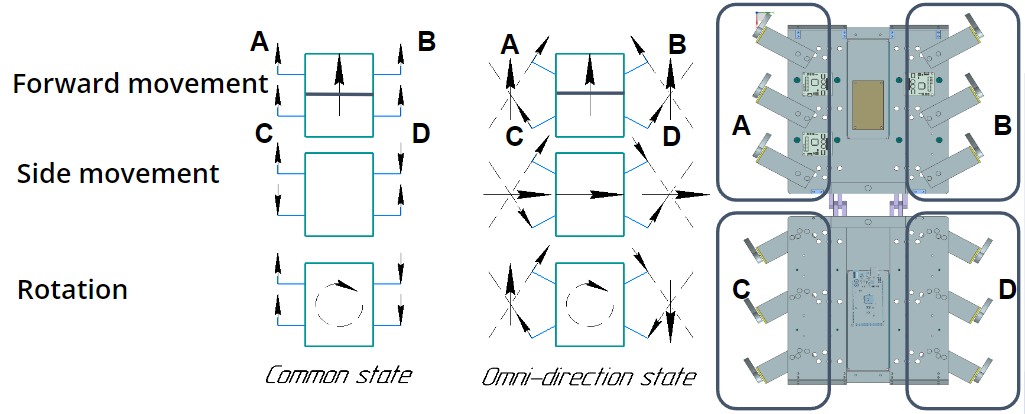
\includegraphics[height=10cm,width=1\textwidth,keepaspectratio]{omni_rot.png}
    \caption{Векторное представление сил в классическом и всенаправленном состоянии}
    \label{fig:omnidirection}
\end{figure}

На рисунке \ref{fig:omnidirection} представлена иллюстрация данной концепции: для того, чтобы робот двигался во всех направлениях, необходимо разбить ноги на группы, чтобы получилось 4 группы A-D.

Если сравнивать с классической компоновкой роботов (угол между корпусом робота и осью вала привода ноги равен 90 градусов), то вектор внешних сил будет таким, как на левой части рис. \ref{fig:omnidirection}. Стрелка в центре робота — суперпозиция всех сил. Если изменить угол оси привода ноги в соответствии с предлагаемой концепцией, то возможно получить значения суперпозиции сил, представленные на рис. \ref{fig:omnidirection} в центре. То есть, чтобы переместить корпус робота направо, группы А и D должны вращать ноги в одну сторону, а группы C и B — в противоположную. Правая часть рисунка иллюстрирует расположение групп ног на исследуемом роботе. 

В рамках исследования было разработано четыре концепции робота СтриРус. В таблице \ref{tabular:robot_comparison} в строке недостатки объясняются основные причины перехода из одной итерации к другой. Концептуально было замечено, что высота ноги и наличие сегмента разительно влияет на проходимость конструкции. \quad \qrcode[height=1.5cm]{https://youtu.be/EQ6oGZVDpoc}

\begin{figure}[H]
    \centerfloat{
        \hfill
        \subcaptionbox[List-of-Figures entry]{Первая итерация\label{fig:strirus_0}}{%
            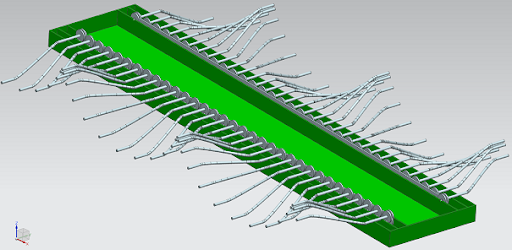
\includegraphics[width=0.49\linewidth]{strirus_0.png}}
        \hfill
        \subcaptionbox[List-of-Figures entry]{Вторая итерация \label{fig:strirus_1}}{%
            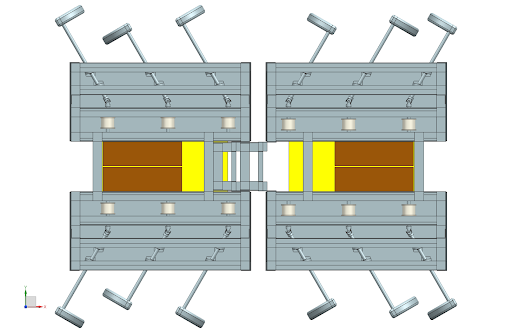
\includegraphics[width=0.49\linewidth]{strirus_1.png}}

        \hfill
        \subcaptionbox{Третья итерация\label{fig:strirus_2}}{%
        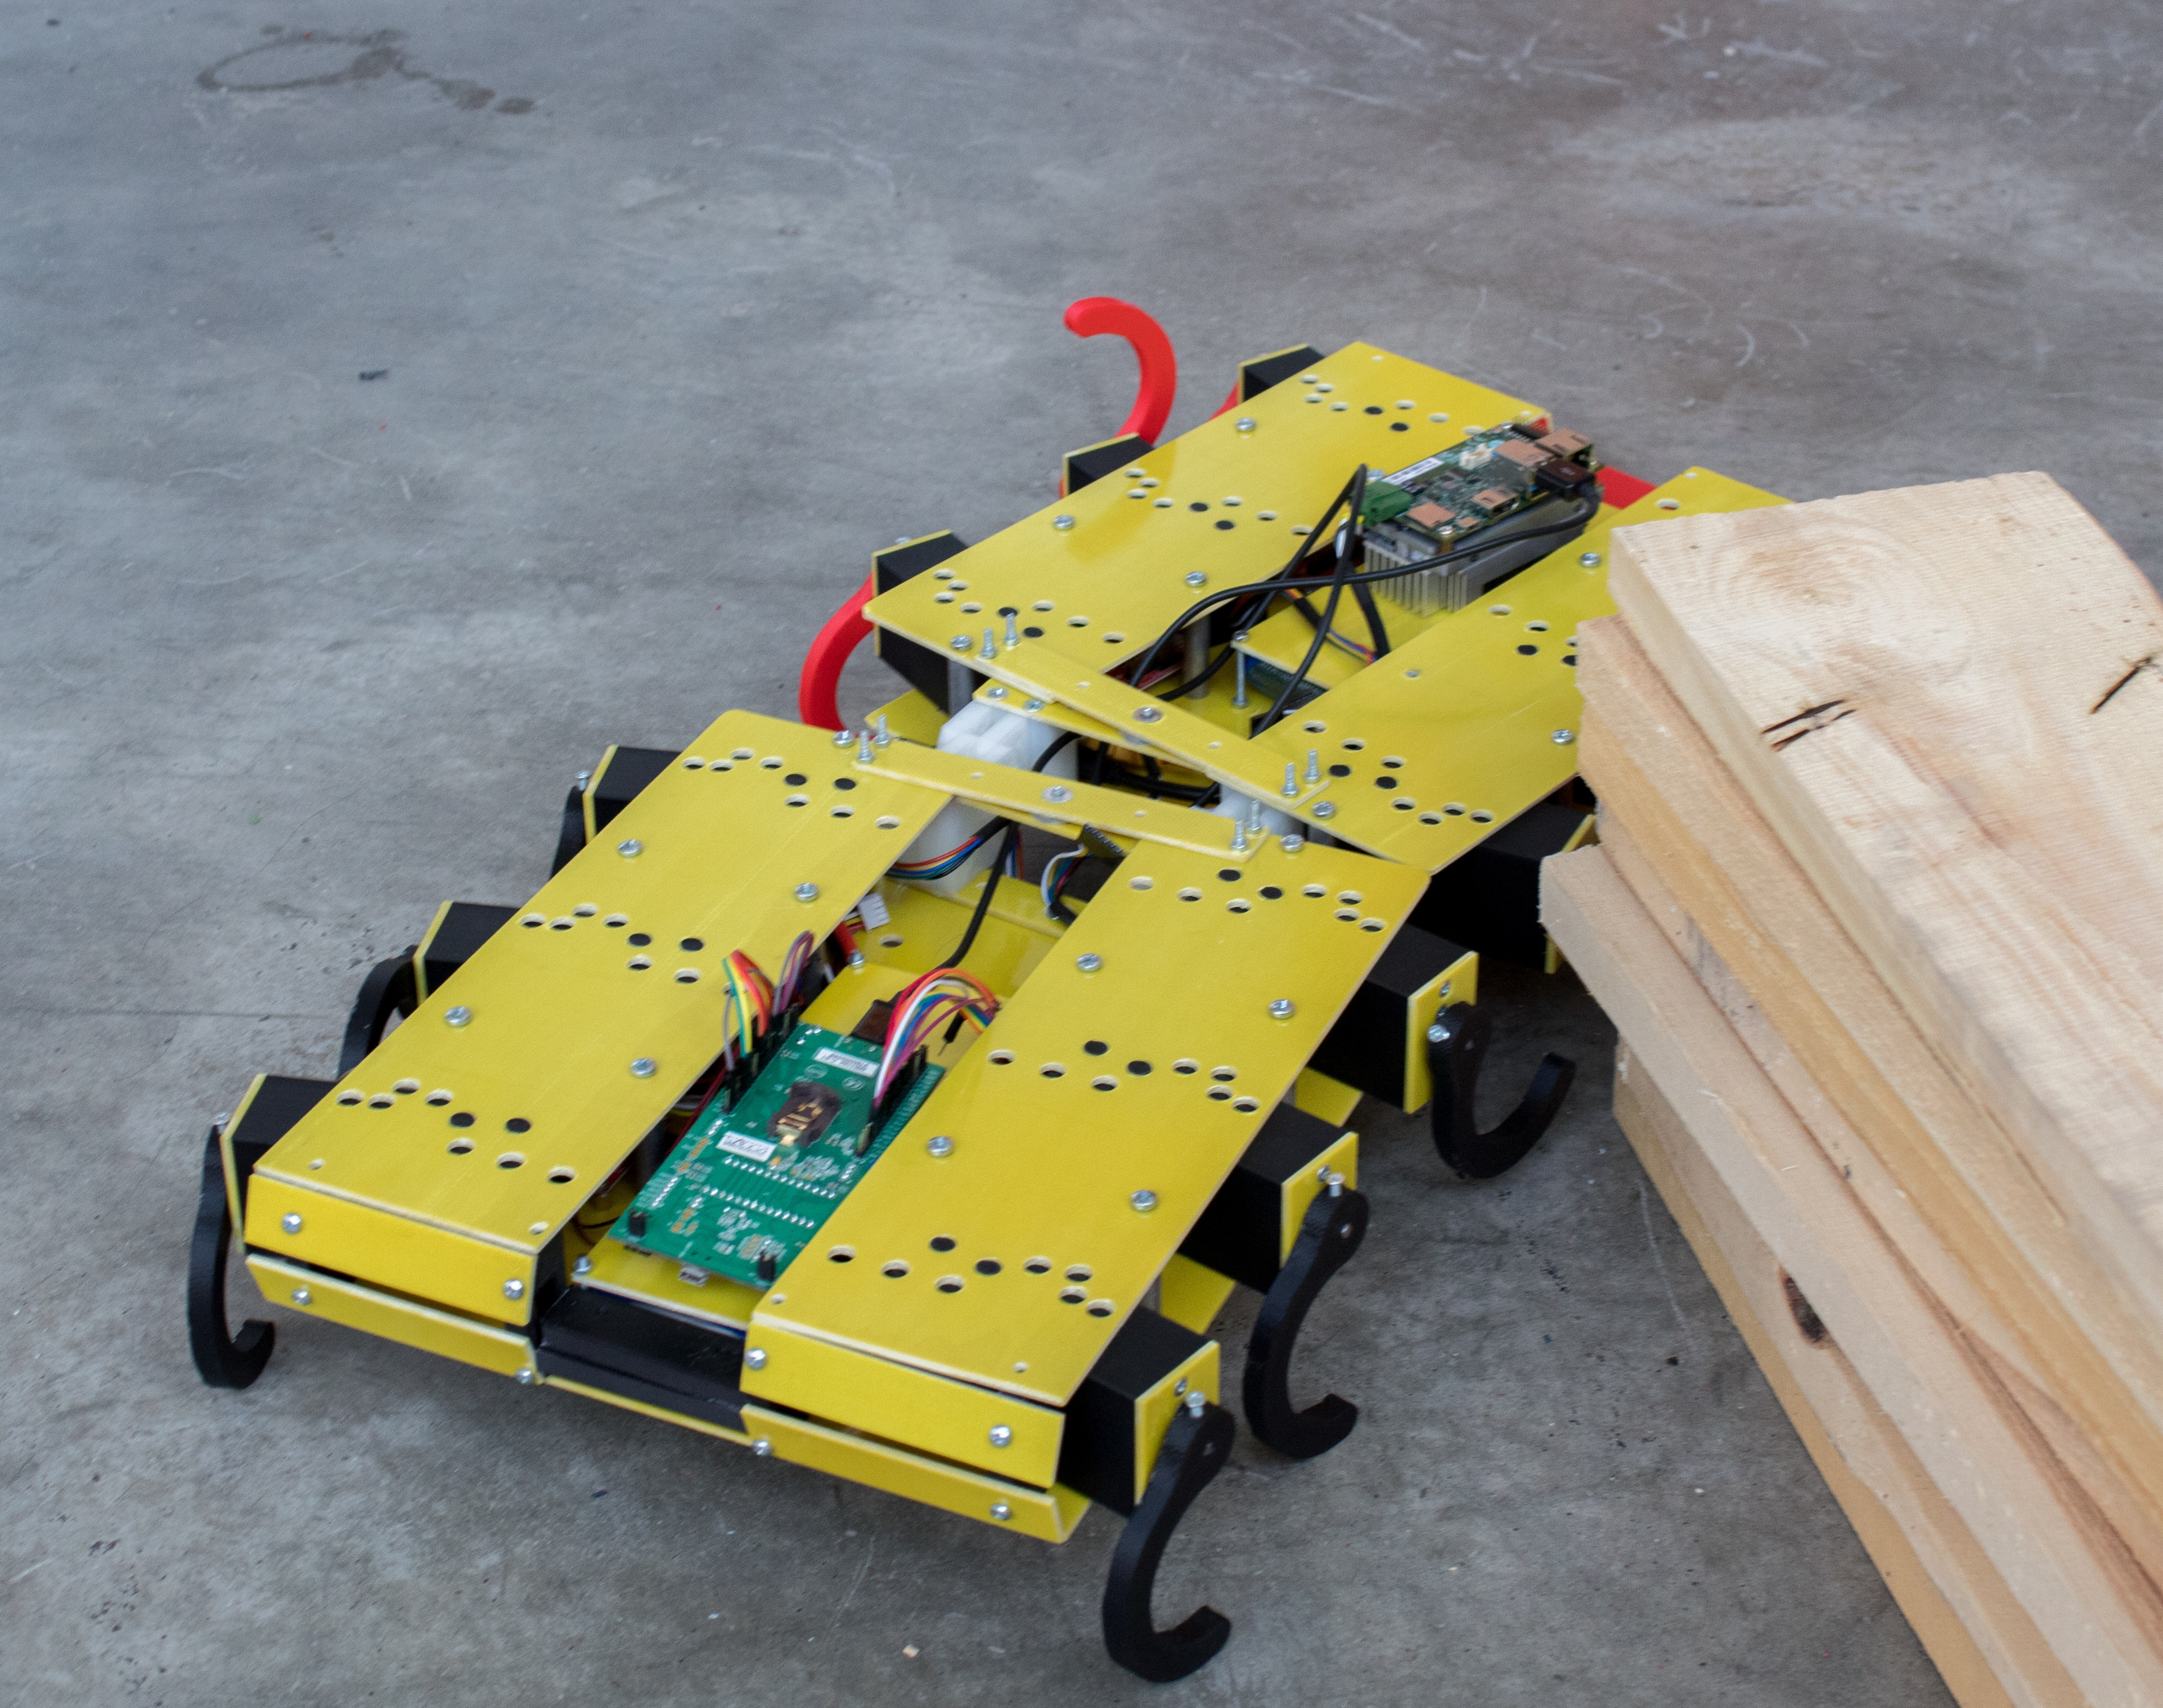
\includegraphics[width=0.49\linewidth]{strirus_2.jpg}}
        \hfill
        \subcaptionbox{Третья итерация, улучшенная\label{fig:strirus_3}}{%
        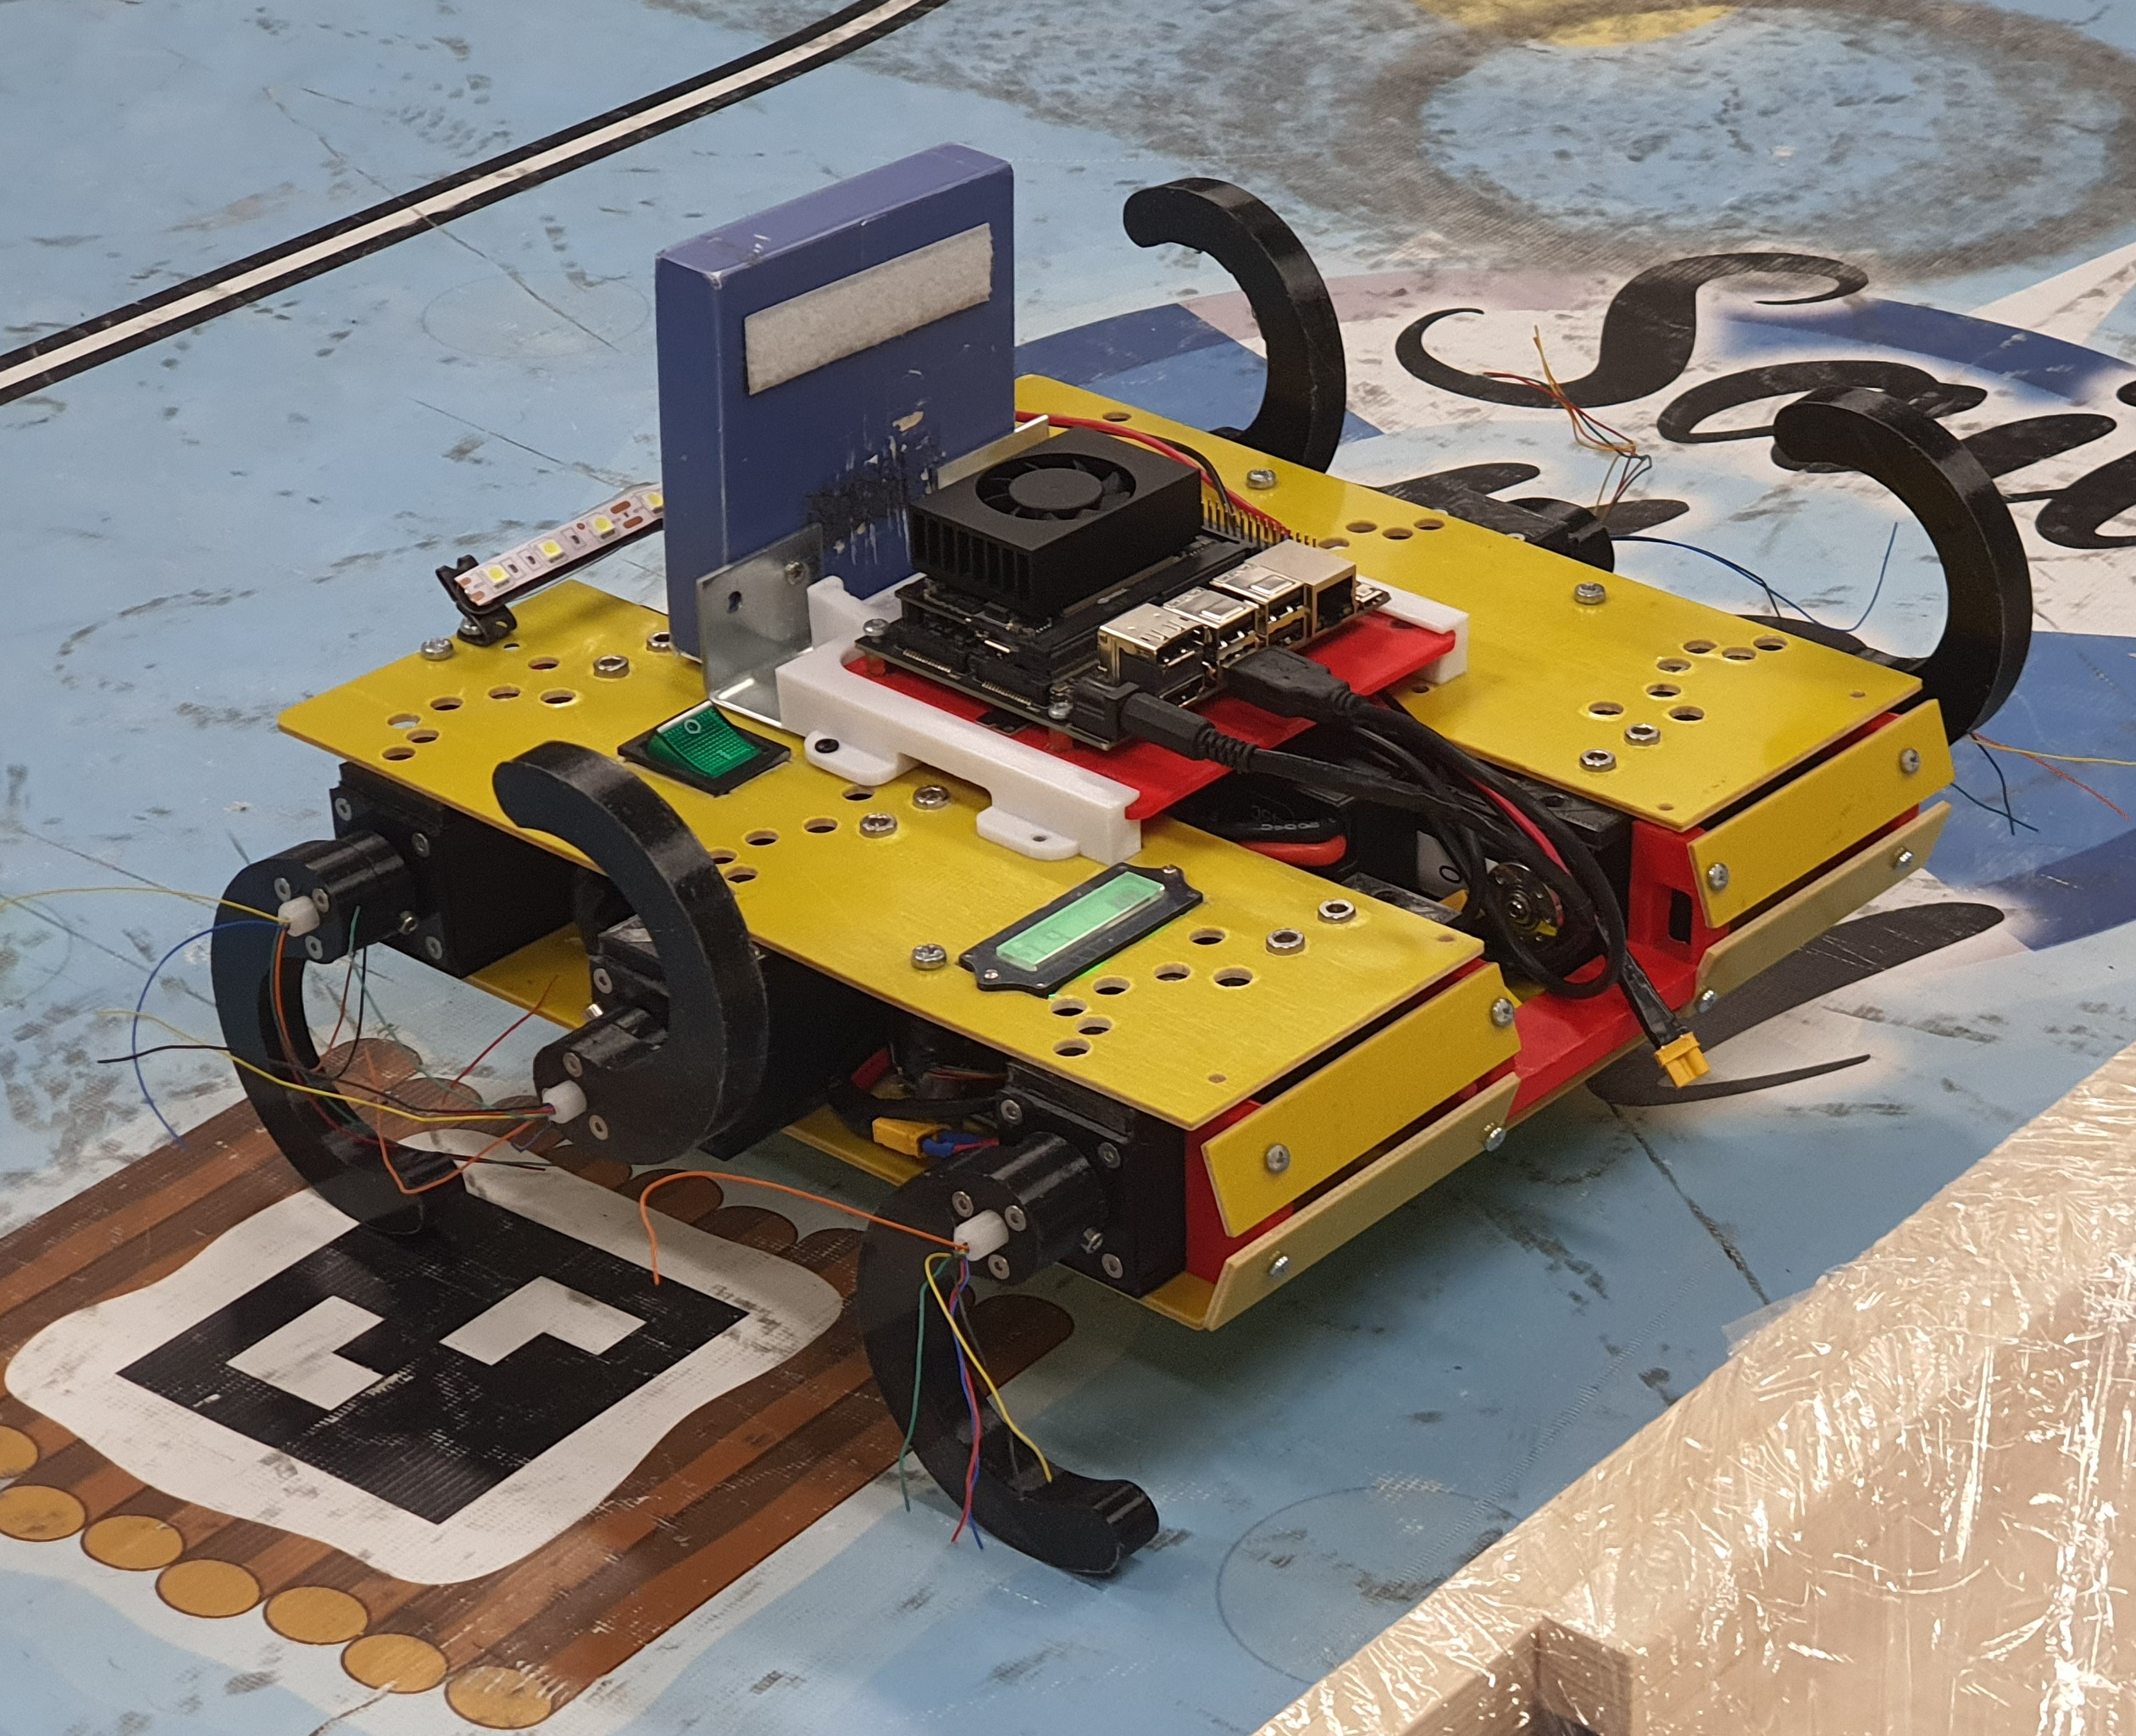
\includegraphics[width=0.49\linewidth]{strirus_3.JPG}}
        \hfill

        \subcaptionbox{Четвертая итерация\label{fig:strirus_4}}{%
        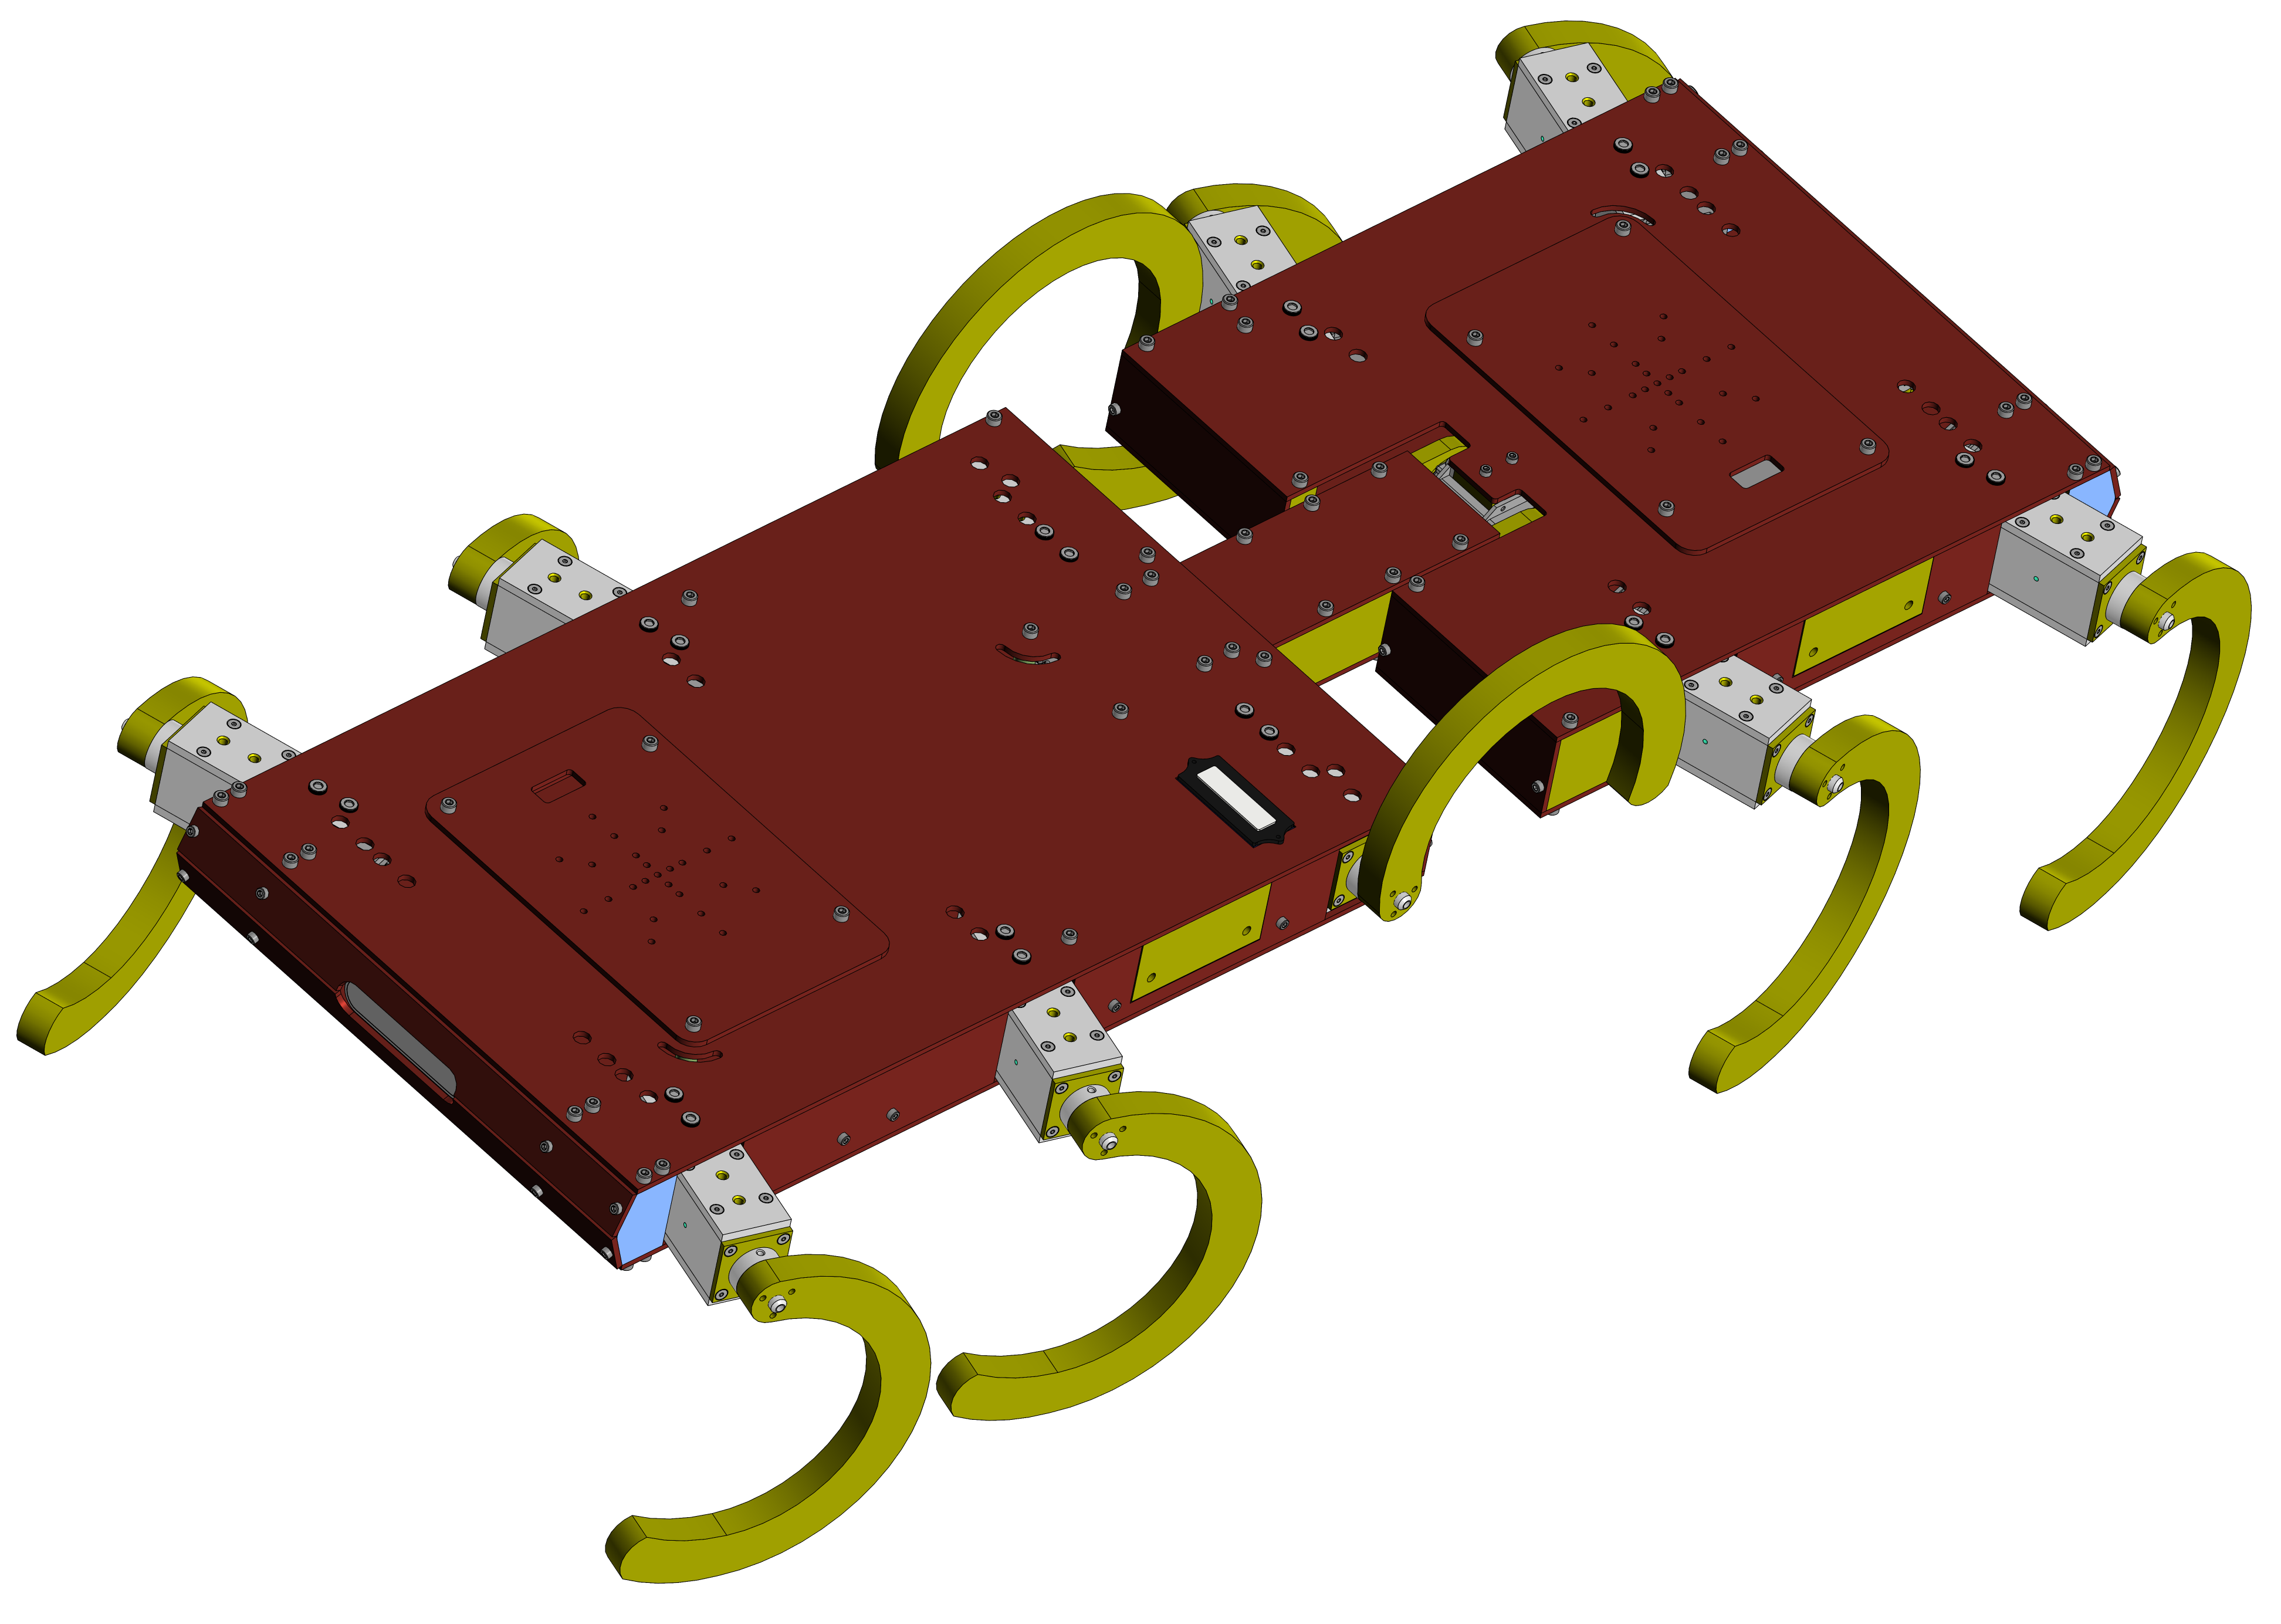
\includegraphics[width=0.9\linewidth]{strirus_4.png}}
    }
    % \legend{Подрисуночный текст, описывающий обозначения, например. Согласно
    %     ГОСТ 2.105, пункт 4.3.1, располагается перед наименованием рисунка.}
    \caption{Итерации робота СтриРуса}\label{fig:striruses}
  \end{figure}

\begin{table}[H]
    \caption{Сравнение итераций робота}
    \label{tabular:robot_comparison}
    % \begin{center}
    \begin{footnotesize}
    \begin{tabular}{p{1.6cm}|p{2cm}|p{2cm}|p{2cm}|p{2cm}|p{2cm}}
    \toprule
    \toprule
    % \rowcolor{Gray}
     Итерация & 1 \pic{fig:strirus_0}  & 2 \pic{fig:strirus_1} &  3 \pic{fig:strirus_2} & 3+ \pic{fig:strirus_3} & 4 \pic{fig:strirus_4} \\
     \hline
     Кол-во ног & 54 & 12 & 12 & 6 & 10 \\ 
    %   \rowcolor{lightgray}
     \makecell[l]{Кол-во \\ сегментов} & 1 & 2 & 2 & 1 & 2 \\
     \makecell[l]{Тип \\ соединения} & --- & Тангаж & \makecell[l]{Тангаж,\\ рыскание} & --- & Тангаж \\
    %  \rowcolor{lightgray}
     Отн. угол телом -- нога, градусы & 0 & 0--45 & 0, 15, 30, 45 & 0 & 0, 15 \\
     \makecell[l]{Высота \\ ноги, мм} & 54 & 60 & 60 & 90 & 170 \\
     \hline
     Особенности & Волноход & Механизм, который позволяет непрерывно изменять отн. угол & Двухстепенной узел, соединяющий сегменты & Большие ноги & Гигантские ноги  \\
    %  \rowcolor{lightgray}
    \hline
     Недостатки & Невозможно установить сенсоры на ноги. Много подвижных частей & Слишком сложный механизм, изменяющий отн. угол & Мал. ноги. Избыточная вторая степень свободы в соединительном узле & 1 сегмент. Маленькие ноги & --- \\
    \bottomrule
    \bottomrule
    \end{tabular}
    \end{footnotesize}
    % \end{center}
    \end{table}

Как итог, был разработан 10 ногий двух сегментный робот СтриРус. 10 ног было выбрано на основе результатов, полученных во время решения мультикритериальной задачи оптимизации с помощью генетического алгоритма.

Конструкция робота соответствует всем требованиям, поставленным вначале. А именно, возможность проходить сквозь узкие пространства, иметь возможность преодолевать большие каменные гряды и возможность эффективно перемещаться по сыпучим грунтам.


